\documentclass[aspectratio=169]{beamer}
% \setbeamertemplate{footline}[frame number]
\usepackage{color,amsmath}
\usepackage{subfigure}
\usepackage{booktabs}
\usepackage{framed}
\usepackage{comment}
\hypersetup{
colorlinks=true,
linkcolor=blue,
filecolor=magenta,      
urlcolor=blue,
pdftitle={Overleaf Example},
pdfpagemode=FullScreen}
\usepackage{tabularx}

%%%%%%%%%%%%%%%%%%%%%%%%%%
\title[]{Survey research in the digital age}
\author[]{Bernhard Clemm von Hohenberg\\Department of Computational Social Science\\GESIS}
\date[]{Summer Institutes in Computational Social Science\\July 28, 2023}
\begin{document}
%%%%%%%%%%%%%%%%%%%%%%%%%%
\frame{\titlepage}
%%%%%%%%%%%%%%%%%%%%%%%%%%
\begin{frame}{Schedule}

\vspace{0.5em}
\begin{itemize}
\item 9.00-9.45 Introduction \& total error survey framework
\item 9.45-10.15 Probability and non-probability sampling
\vspace{0.5em}
\item Coffee break
\vspace{0.5em}
\item 10.30-11.00 Computer-administered interviewing
\item \textcolor{violet}{11.00-11.30 Linking surveys to big data}
\item 11:30-13:00 Intro and begin group exercise
\vspace{0.5em}
\item Lunch (or Eisbach plunge)
\vspace{0.5em}
\item 14:00-15:45 Continue group exercise
\end{itemize}

\end{frame}
%%%%%%%%%%%%%%%%%%%%%%%%%%%
\begin{frame}{Credits}

These materials build heavily on Matthew Salganik's 2019 SICSS class as well as Chapter 3 of ``Bit by Bit: Social Research in the Digital Age''.

\end{frame}
%%%%%%%%%%%%%%%%%%%%%%%%%%%
\begin{frame}
\begin{center}
\renewcommand{\arraystretch}{1.5}
\begin{tabular}{p{0.1\textwidth}p{0.26\textwidth}p{0.24\textwidth}p{0.24\textwidth}}
& \textbf{Sampling} & \textbf{Interviews} & \textbf{Data environment}\\
\hline \hline
1st era & Area probability & Face-to-face & Stand-alone \\
\hline
2nd era & Random digital dial probability & Telephone & Stand-alone \\
\hline
3rd era & Non-probability & Computer-administered  & \textcolor{violet}{Linked} \\
\end{tabular}
\end{center}

\end{frame}
%%%%%%%%%%%%%%%%%%%%%%%%%%%
\begin{frame}

\begin{center}
\LARGE{Will big data kill surveys?}
\end{center}

\end{frame}
%%%%%%%%%%%%%%%%%%%%%%%%%%%%%
\begin{frame}

\begin{center}
\only<1>{\includegraphics[width=0.6\textwidth]{figures/peanutbutterlover}}
\only<2>{\includegraphics[width=0.6\textwidth]{figures/peanutbutterlover_bigdata_survey}}
\end{center}

\vfill
\tiny{\url{http://schlitterblog.com/wp-content/uploads/2014/05/peanutbutterlover.jpg}}

\end{frame}
%%%%%%%%%%%%%%%%%%%%%%%%%%%
\begin{frame}{Overview}

\begin{center}
\includegraphics[width=0.7\textwidth]{figures/bitbybit3-12_found_survey_combined.png}
\end{center}

\end{frame}
%%%%%%%%%%%%%%%%%%%%%%%%%%%
\begin{frame}

\begin{center}
\LARGE{Enriched asking} \\
\end{center}
Survey data builds context around a big data source (or vice versa) that contains some important measurements but lack others. 

\textbf{}: 

\end{frame}
%%%%%%%%%%%%%%%%%%%%%%%%%%%
\begin{frame}

\begin{center}
\includegraphics[width=0.8\textwidth]{figures/guess2021.png}
\end{center}

\vfill
\tiny{\url{https://onlinelibrary.wiley.com/doi/full/10.1111/ajps.12589}}

\end{frame}
%%%%%%%%%%%%%%%%%%%%%%%%%%%
\begin{frame}

\begin{center}
\only<1>{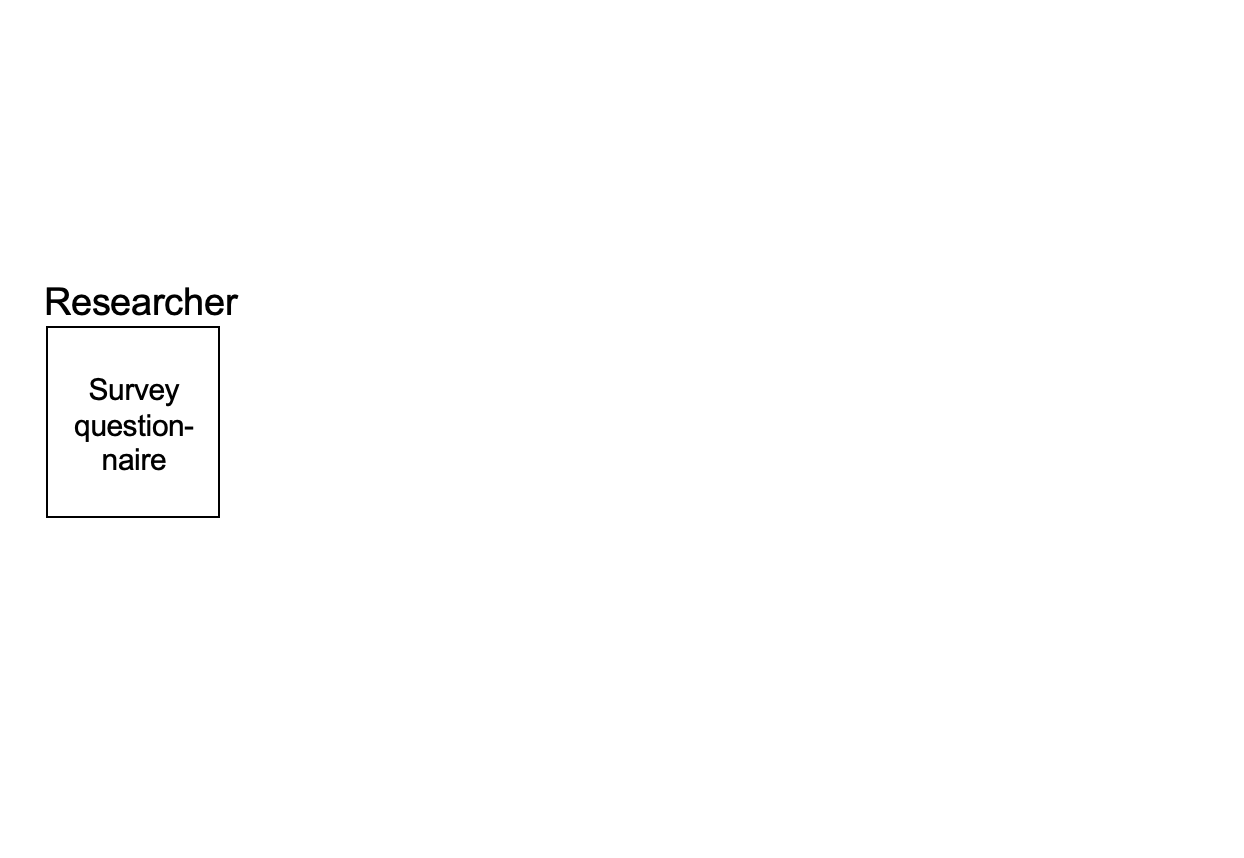
\includegraphics[width=0.8\textwidth]{figures/guess2021-schematic-1.png}}
\only<2>{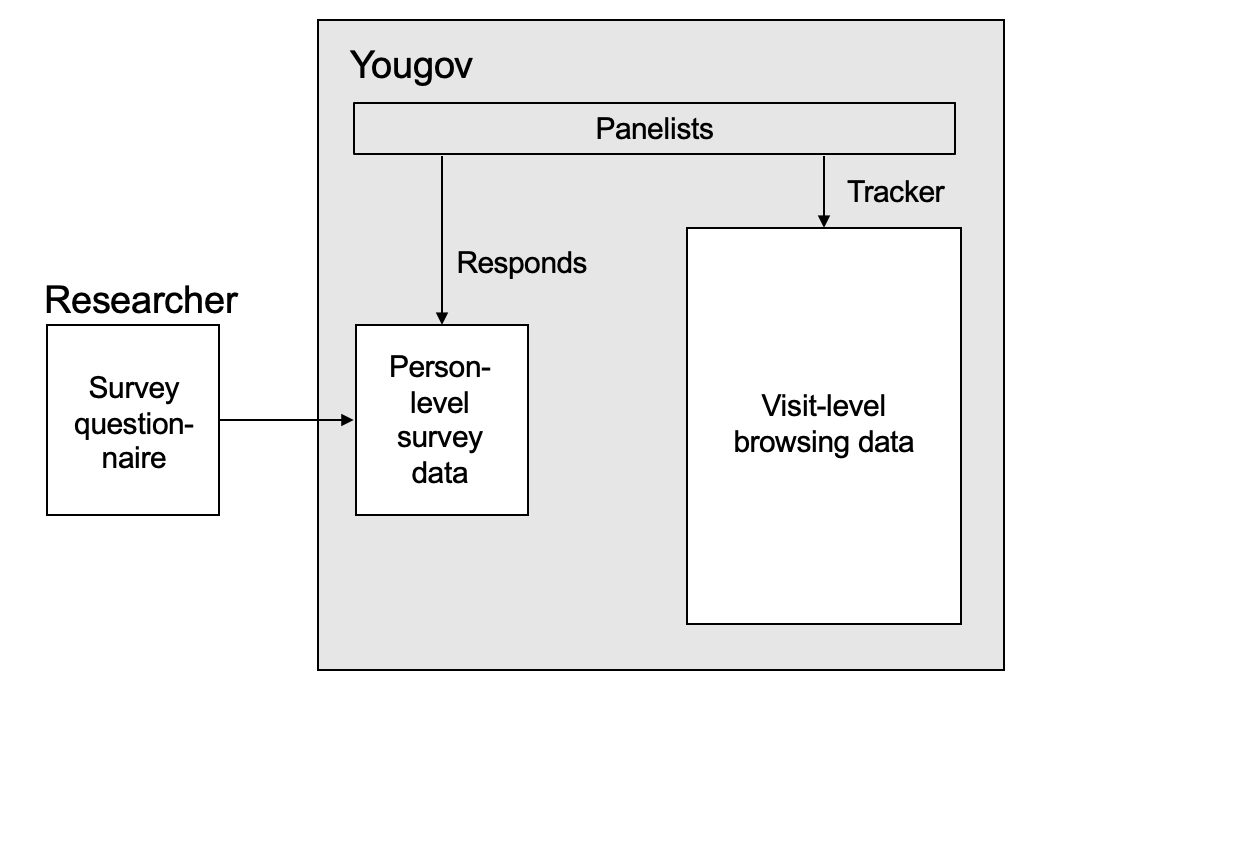
\includegraphics[width=0.8\textwidth]{figures/guess2021-schematic-2.png}}
\only<3>{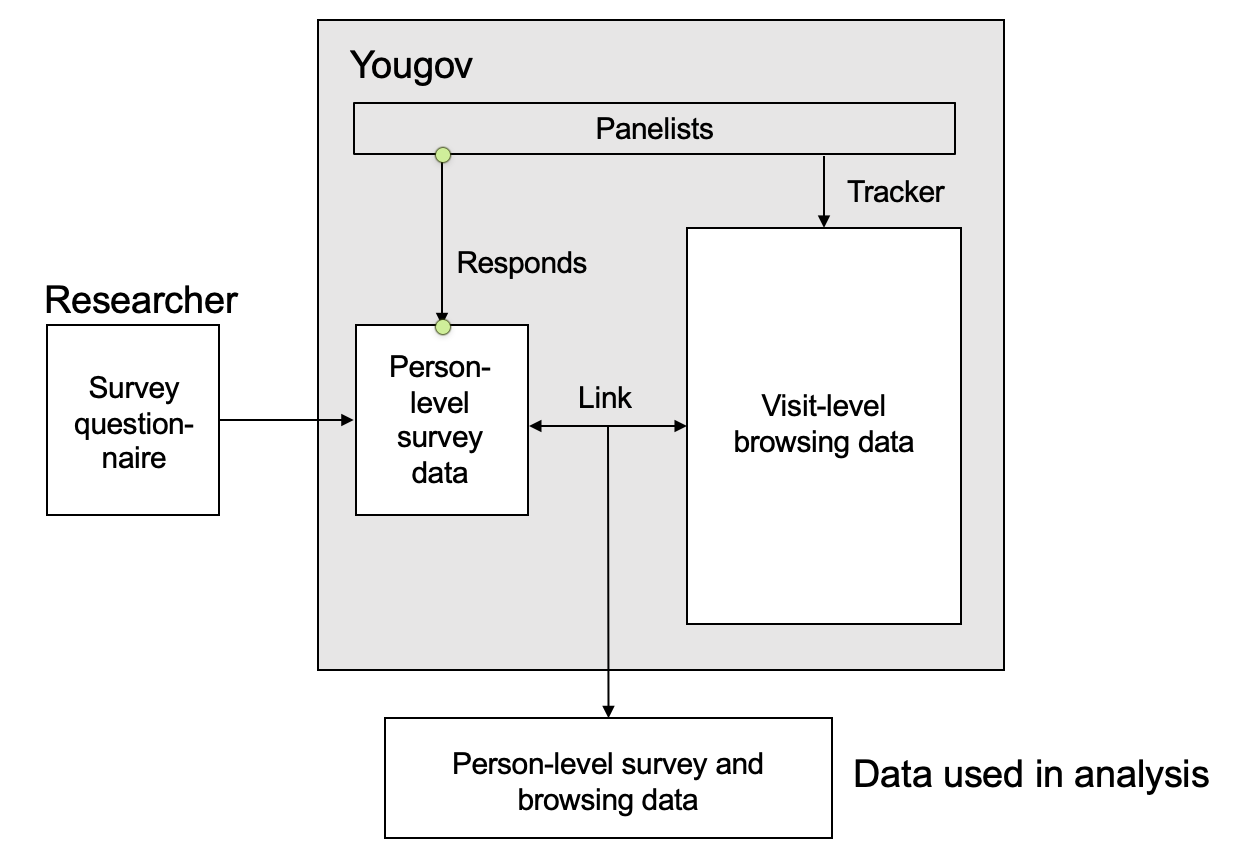
\includegraphics[width=0.8\textwidth]{figures/guess2021-schematic-3.png}}
\end{center}

\end{frame}
%%%%%%%%%%%%%%%%%%%%%%%%%%%
\begin{frame}

\begin{center}
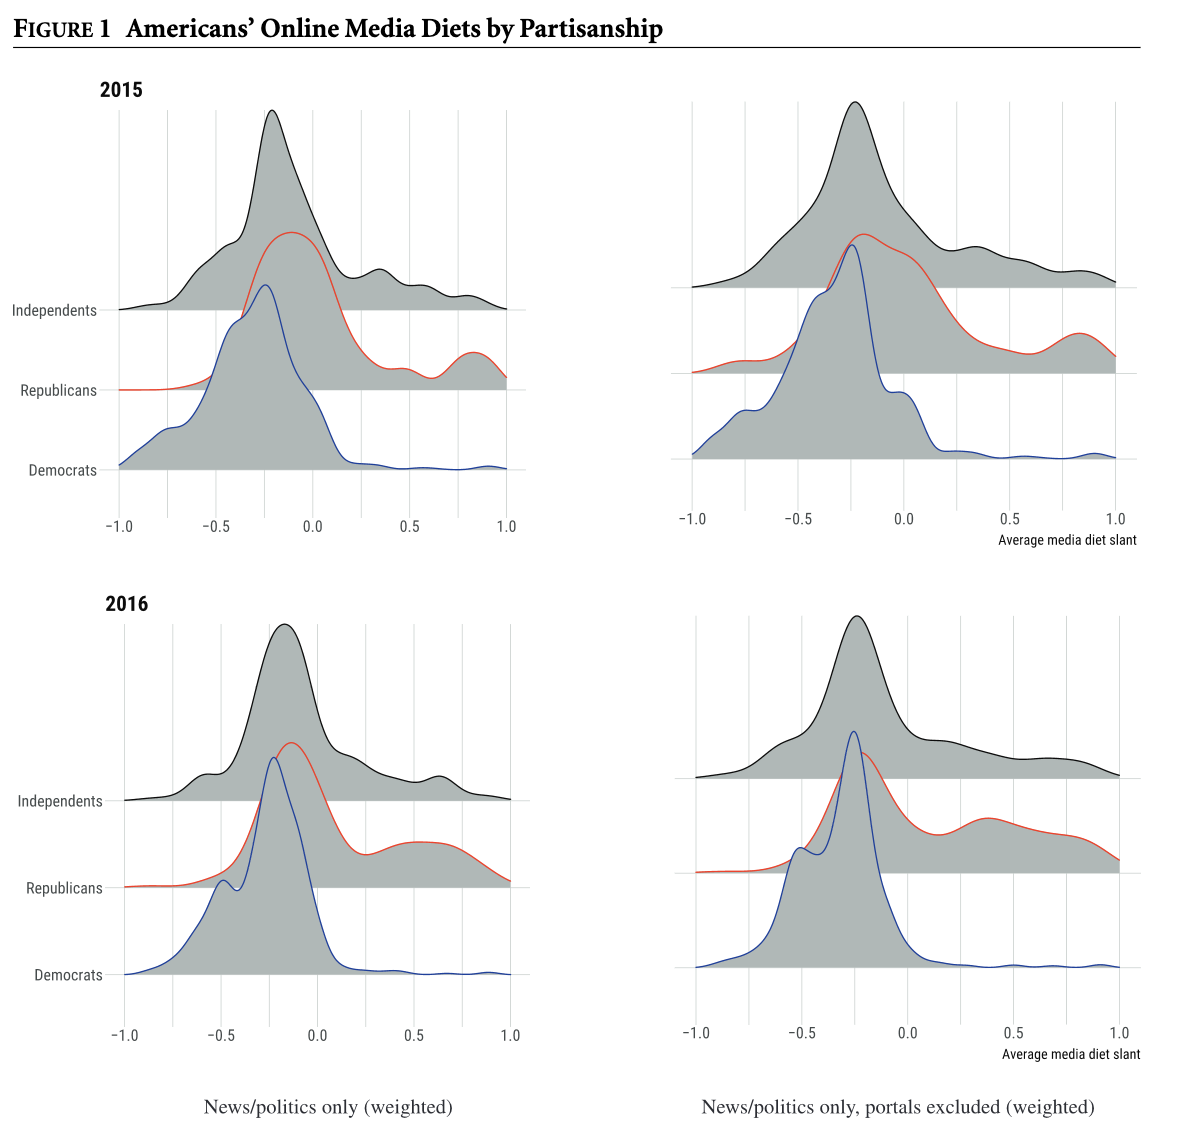
\includegraphics[width=0.62\textwidth]{figures/guess2021-figure1.png}
\end{center}

\end{frame}
%%%%%%%%%%%%%%%%%%%%%%%%%%%
\begin{frame}

Another rising approach: data donations

\begin{center}
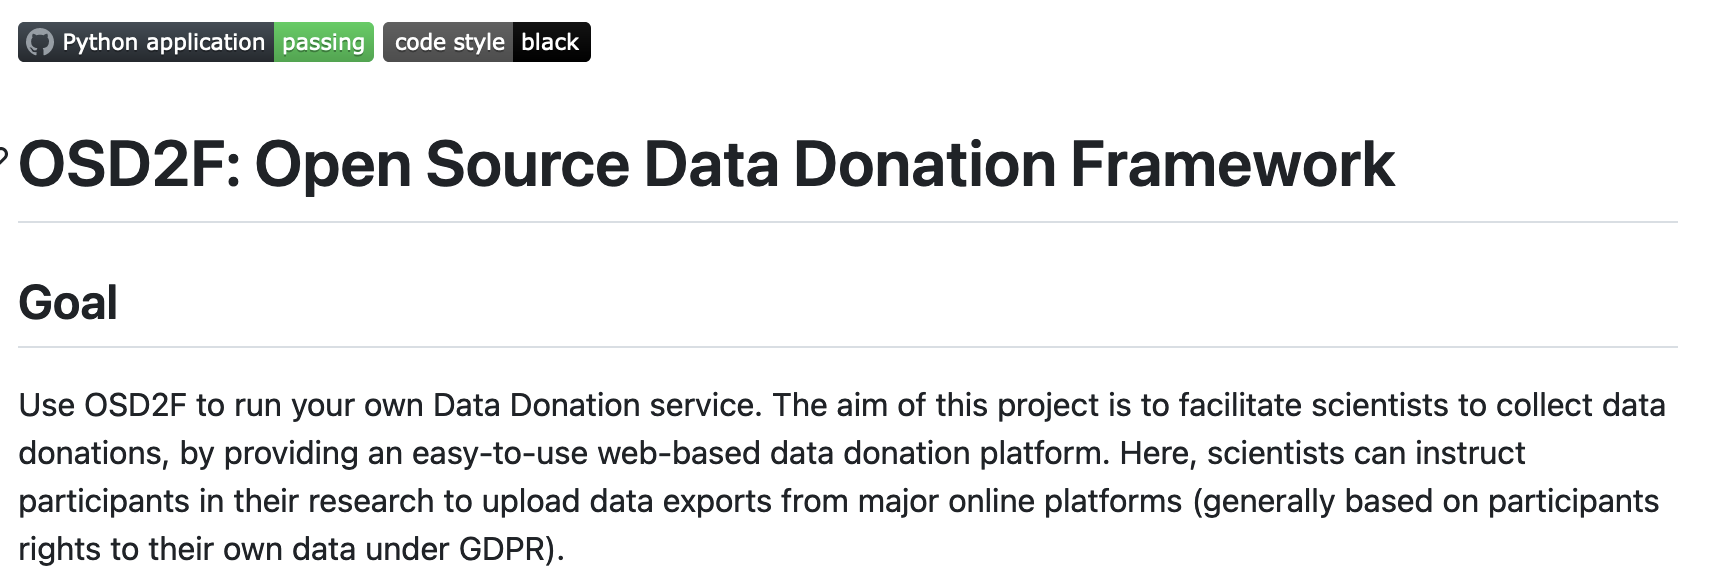
\includegraphics[width=\textwidth]{figures/osd2f.png}
\end{center}

\end{frame}
%%%%%%%%%%%%%%%%%%%%%%%%%%%
\begin{frame}

\begin{center}
\LARGE{Amplified asking} \\
\end{center}
Using a predictive model to combine survey data from a few people with a big data source from many people. 

\end{frame}
%%%%%%%%%%%%%%%%%%%%%%%%%%%
\begin{frame}

\begin{center}
\includegraphics[width=0.8\textwidth]{figures/blumenstock_predicting_2015_title}
\end{center}

\vfill
\tiny{\url{http://dx.doi.org/10.1126/science.aac4420}}
\end{frame}
%%%%%%%%%%%%%%%%%%%%%%%%%%%
\begin{frame}

\begin{center}
\only<1>{\includegraphics[width=0.7\textwidth]{figures/blumenstock_predicting_2015_schematic_1}}
\only<2>{\includegraphics[width=0.7\textwidth]{figures/blumenstock_predicting_2015_schematic_2}}
\only<3>{\includegraphics[width=0.7\textwidth]{figures/blumenstock_predicting_2015_schematic_3}}
\only<4>{\includegraphics[width=0.7\textwidth]{figures/blumenstock_predicting_2015_schematic_4}}
\only<5>{\includegraphics[width=0.7\textwidth]{figures/blumenstock_predicting_2015_schematic_5}}
\only<6>{\includegraphics[width=0.7\textwidth]{figures/blumenstock_predicting_2015_schematic_6}}
\end{center}

\end{frame}
%%%%%%%%%%%%%%%%%%%%%%%%%%%
\begin{frame}

\begin{center}
\includegraphics[width=0.7\textwidth]{figures/blumenstock_predicting_2015_fig1a}
\end{center}

\end{frame}
%%%%%%%%%%%%%%%%%%%%%%%%%%
\begin{frame}

\begin{center}
\includegraphics[width=0.7\textwidth]{figures/blumenstock_predicting_2015_fig2}
\end{center}

\end{frame}
%%%%%%%%%%%%%%%%%%%%%%%%%%
\begin{frame}

\begin{center}
\includegraphics[width=0.45\textwidth]{figures/blumenstock_predicting_2015_fig3c}
\end{center}

\pause

\begin{itemize}
\item 10 times faster
\item 50 times cheaper
\end{itemize}

\end{frame}
%%%%%%%%%%%%%%%%%%%%%%%%%%
\begin{frame}{Summary}


\begin{itemize}
\item Surveys and big data are compliments not substitutes
\pause
\item Sometime we do ``enriched asking'' and sometimes ``amplified asking'' (role of big data source is different in both cases)
\pause
\item The black box of many big-data providers is a challenge for scientists
\end{itemize}

\end{frame}
%%%%%%%%%%%%%%%%%%%%%%%%%%
\begin{frame}

\begin{center}
    Questions
\end{center}

\end{frame}
%%%%%%%%%%%%%%%%%%%%%%%%%%%


\end{document}
